\section{Trusted Setup}
\label{sec:trustedSetup}

A trusted setup is required before anyone can generate a zk-SNARK (`proof') for a particular computation. In Nightfall, there are currently six separate computations for which a trusted setup is required: non-fungible minting, transferring and burning; and fungible minting, transferring and burning.
For each computation, the trusted setup is only performed once; at ``the beginning of time''; by a generous trusted benefactor; and before the \hyperref[sec:smartContracts]{Shield contract} can be deployed to the Ethereum blockchain for people to use. 
In Nightfall it is currently assumed that the generous benefactor will not use secret information obtained in the setup in order to subvert the security of the protocol.

\begin{figure}[h]
	\centering
	\begin{minipage}{0.3\textwidth}
		\centering
		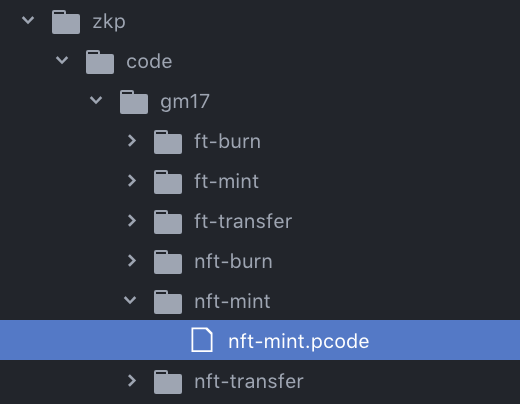
\includegraphics[width=0.7\textwidth]{files-before-setup.png}
	\end{minipage}
	\quad
	\begin{minipage}{0.3\textwidth}
		\centering
		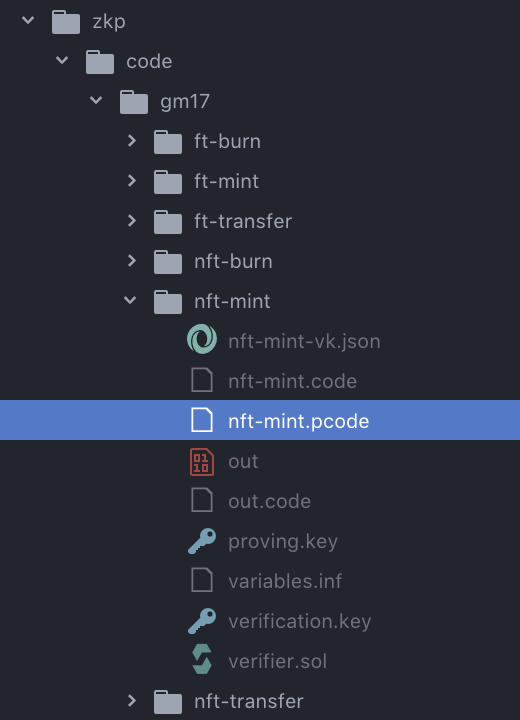
\includegraphics[width=0.7\textwidth]{files-after-setup.png}
	\end{minipage}
	\smallbreak
	\caption{Files in $\mathcal{T}$'s local repository before (left) and after (right) performing a trusted setup.}
	\label{pic:filesBeforeAfterSetup}
\end{figure}

The trusted setup abstracts the human-readable code of the ZoKrates DSL (files with a \texttt{.code} or \texttt{.pcode} extension) into a (proving key, verification key) pair.\\
\\
Suppose $\mathcal{T}$ is a `trusted benefactor' who intends to use Nightfall to set up the infrastructure which will allow anyone to transfer ownership of tokens under zero knowledge.
When $\mathcal{T}$ first clones the Nightfall repository, he only has human-readable computations written in \texttt{`.pcode'} syntax. Taking the \texttt{./zkp/code/gm17/nft-mint/} folder as an example, $\mathcal{T}$ will initially only have
\texttt{`nft-mint.pcode'}.  
The trusted setup will provide $\mathcal{T}$ with:
\texttt{`nft-mint-vk.json'}, \texttt{`nft-mint.code'},
\texttt{`out'}, \texttt{`out.code'}, \texttt{`proving.key'},
\texttt{`variables.inf'}, \texttt{`verification.key'},
\texttt{`verifier.sol'}.
This is shown in Figure~\ref{pic:filesBeforeAfterSetup} and a brief explanation of each of these files is provided in Table~\ref{table:trustedoutput}.

\begin{table}[h]
	\begin{center}
		\begin{tabular}[t]{L{0.2\textwidth}L{0.7\textwidth}}
			\toprule
			Trusted Setup Output & Explanation  \\ \midrule 
			\texttt{nft-mint-vk.json} & The verification key for an `nft-mint'. This will be stored on-chain, within the \hyperref[sec:smartContracts]{Verifier Registry}. Every time a user submits a (proof, public inputs) pair to the \hyperref[sec:smartContracts]{Shield contract}, this pair is verified with respect to the verification key within the \hyperref[sec:smartContracts]{Verifier contract}.
			\\
			\texttt{nft-mint.code} & Human-readable computation for an `nft-mint', written in the DSL of ZoKrates.
			\\
			\texttt{nft-mint.pcode} & An abbreviation of the \texttt{.code} syntax, for easier writing.
			\\
			\texttt{out} & Ignore. \\
			\texttt{out.code} & Ignore 
			\\
			\texttt{proving.key} & Used to generate proofs. Every time a User generates a new proof, this file is used by ZoKrates. 
			\\
			\texttt{variables.inf} & Ignore 
			\\
			\texttt{verification.key} & A representation of the verification key. Nightfall uses the jsonified version of the verification key (\texttt{mint-nft-vk.json}) and submits it as a flattened array to the \hyperref[sec:smartContracts]{Verifier Registry}.
			\\
			\texttt{verifier.sol} & Ignore.  This is an example implementation of a verifier contract with the verification key hard-coded into it.  It is unused by Nightfall. \\ \bottomrule
		\end{tabular}
	\end{center}
\caption{The files output by the trusted setup.}
\label{table:trustedoutput}
\end{table}

\textbf{Remark:}
The proving keys are by far the largest files required by Users of Nightfall:
\begin{center}
\begin{tabular}{ll}
	nft-mint & 77 MB\\
	nft-transfer & 1.1 GB\\
	nft-burn & 1.0 GB\\
	ft-mint & 77 MB\\
	ft-transfer & 2.1 GB\\
	ft-burn & 1.0 GB\\
\end{tabular}
\end{center}

The file sizes shown here reflect the sizes of the files once extracted from a ZoKrates container and stored on a User's local machine. (As opposed to the proving key sizes displayed in Table~\ref{table:efficiency}, which are calculated at setup time). The `transfer' and `burn' proving keys are particularly large, because of how a User proves that their token commitment exists as a leaf of the on-chain Merkle Tree (see \hyperref[part:theProtocols]{The Protocols}). As a default size, the on-chain Merkle Tree is 33-deep, meaning $32$ sha256 hashes are performed to calculate the root of the Merkle Tree from the relevant leaf. Each sha256 hash requires around $25,000$ constraints. For a fungible transfer, $64$ sha256 hashes are performed ($2 \times 32$).

Once $\mathcal{T}$ has completed the trusted setup for each of the six computations, he is ready to create the rest of the Nightfall infrastructure.
We outline his steps in Figure~\ref{fig:trustedSetup}. The Smart Contracts being alluded to are discussed in more detail in the \hyperref[sec:smartContracts]{Smart Contracts} section.
\begin{figure}[ht]
	\begin{center}
		\begin{framed}
      \begin{tabular}{p{16cm}}	
        \textbf{Deploying the Nightfall Infrastructure} \\ \midrule
         \\
        \textbf{Trusted Benefactor steps}:
        \begin{enumerate}
				  \item Perform the `Trusted Setup' to produce the proving key and the verification key for each of the six computations.
				  \item Share the proving keys with the world (e.g. through an online sharing service). Do not share the proving keys on a blockchain; they're way too big!
				  \item Locate the Verifier Registry contract's address on the Ethereum mainnet. We intend there to only be one Verifier Registry on the mainnet for all zk-SNARK traffic; in much the same way as the ENS registers all .eth domain names. Note, however, that the default migration scripts of the Nightfall repository do deploy an instance of a Verifier Registry, for example's sake.
          \item Either:
          \begin{itemize}
            \item Locate a GM17 verifier contract address on the Ethereum mainnet; or
            \item Deploy an instance of the GM17 verifier contract to the Ethereum mainnet. And register this GM17 verifier contract with the Verifier Registry (see \texttt{./zkp/src/vk-controller.js} which does this in the Nightfall repository).
          \end{itemize}
          \item Choose which ERC-20 token you wish for your new infrastructure to `shield'.
          \item Deploy an instance of the \texttt{FTokenShield.sol} contract to the Ethereum mainnet; specifying the addresses of the chosen GM17 verifier contract and chosen the ERC-20 contract, in the \texttt{constructor} of \texttt{FTokenShield.sol}.
          \item Choose which ERC-721 token you wish for your new infrastructure to `shield'.
          \item Deploy an instance of the \texttt{NFTokenShield.sol} contract to the Ethereum mainnet; specifying the addresses of the chosen GM17 verifier contract and chosen the ERC-721 contract, in the \texttt{constructor} of \texttt{NFTokenShield.sol}.
          \item Store all six verification keys in the Verifier Registry. (See \texttt{./zkp/src/vk-controller.js} which does this in the Nightfall repository). You will receive six \texttt{`vkId'} values from the Verifier Registry in return. These are unique identifiers for the six verification keys.
          \item Share the six \texttt{`vkId'} values with the world; (e.g. through the same online sharing service as the proving keys). It must be clear to Users which vkId corresponds to which proving key. \texttt{./zkp/src/\hyperref[sec:zkp]{vkIds.json}} gives an example of how to store these.
          \item Share the Ethereum addresses of the FtokenShield.sol and NFTokenShield.sol contracts.
          
          \setcounter{ongoingEnumCounter}{\value{enumi}}
        \end{enumerate}
        \ \\
        \midrule \\
        \textbf{User steps}:
        \begin{enumerate}
          %resume counter
          \setcounter{enumi}{\value{ongoingEnumCounter}}
          \item Download each proving key and its corresponding vkId from $\mathcal{T}$'s online sharing portal.
          \item Generate a \texttt{(proof, inputs)} pair, as explained in \hyperref[part:theProtocols]{The Protocols}.
          \item Submit the \texttt{(proof, inputs)} pair to the relevant Shield contract.
          
          E.g., using web3: \texttt{nfTokenShield.mint(proof, inputs, vkId)}
          \item Store relevant data in local database.
          \setcounter{ongoingEnumCounter}{0}
        \end{enumerate}
			\end{tabular}
		\end{framed}
	\end{center}
\caption{Deploying the Nightfall Infrastructure}
\label{fig:trustedSetup}
\end{figure}


\subsection*{Notes for a User}
Ordinary Users of a Nightfall infrastructure do not need to (and should not!) perform a trusted setup themselves. Only the original creator of the Shield contracts needs to.
The trusted setup involves a source of randomness and the (proving key, verification key) pair for a given computation will change each time the trusted setup is performed.
Therefore, if a User wishes to generate 'proofs' (zk-SNARKs) to be verified against a verification key which has been stored on the Ethereum mainnet, they should use the exact proving key and vkId which was generated by the trusted setup and shared with everyone.

To explain further, note that for each verification key stored on-chain, there is a corresponding and unique proving key which was generated at the same time, from the same randomness. It is this proving key which Users must use to generate proofs.
Using any other key the User's proofs will not verify against the verification key which has been stored on-chain.
If a User wishes to generate a proof against an existing, already-deployed verification key, they will need to request the corresponding proving key from the creator of the verification key.

\begin{figure}[H]
  \begin{center}
    \begin{mdframed}[backgroundcolor=verylightred]
      \noindent
      SECURITY WARNINGS 
        \begin{itemize}
          \item[--] Performing the initial 'trusted setup' of a computation -- to convert a \texttt{.code} file into a (proving key, verification key) pair -- requires the generation of some random numbers.\\
          \\
          Once the (proving key, verification key) pair has been generated from the \texttt{.code} file, these random numbers MUST be destroyed. These random numbers MUST never be stored by the party who performed the trusted setup, or that party would be able to generate false proofs which verify as \texttt{true}. These random numbers are often referred to as `toxic waste'.\\
          \\
          Nightfall leverages ZoKrates to perform the trusted setup, and relies on the proper management of the toxic waste by ZoKrates.\\
          \\
          A criticism of zk-SNARKs is that future users of a (proving key, verification key) pair, will have to trust that the party who performed the trusted setup (at the `beginning of time') did so properly and truthfully. 
        \end{itemize} 
    \end{mdframed} 
  \end{center}
  \caption{Security warning: Toxic Waste}
  \label{fig:trustedSetupWarning}
\end{figure}


\begin{center}
  \begin{mdframed}[backgroundcolor=verylightblue]
    Where to look?\\
    \\
    \begin{tabular}{lp{14cm}}
      \texttt{./zkp/code/gm17/nft-mint/nft-mint.pcode} & \texttt{.pcode} files with human-readable computations.\\
      \texttt{./zkp/code/gm17/nft-mint/nft-transfer.pcode} & \\
      \texttt{./zkp/code/gm17/nft-mint/nft-burn.pcode} & \\
      \texttt{./zkp/code/gm17/nft-mint/ft-mint.pcode} & \\
      \texttt{./zkp/code/gm17/nft-mint/ft-transfer.pcode} & \\
      \texttt{./zkp/code/gm17/nft-mint/ft-burn.pcode} & \\
      \texttt{./zkp/code/README-tools-trusted-setup.md} & README for automating the trusted setup.\\
      \texttt{./zkp/code/README-manual-trusted-setup.md} & README for manually performing the trusted setup.\\
      \url{https://github.com/Zokrates/ZoKrates} & ZoKrates source code\\
      \url{https://zokrates.github.io} & ZoKrates documentation\\
      \texttt{./zkp/code/README-tools-code-preprop.md} & explanation of \texttt{.pcode} syntax\\
      \url{https://github.com/EYBlockchain/zokrates-preprocessor} & how to manually transpile from \texttt{.pcode} to \texttt{.code}\\ 
      \texttt{./zkp/code/README-manual-trusted-setup.md} & how to manually do the trusted setup
    \end{tabular}
  \end{mdframed}
\end{center}